\chapter{Background and Motivation}

In this chapter, we summarize the background and motivation underlying this work. In \cref{sec:bm_smt}, we briefly review the approaches to machine translation (MT) and the comparison between them.
\cref{sec:bm_nmt} reviews the formulation of neural machine translation as well as the frameworks utilized to solve the problem.
\cref{sec:bm_tl} discusses transfer learning (TL) as well as its variants.
Finally, \cref{sec:bm_adapters} discusses the adapter module as an alternative methodology for fine-tuning the model and provides reasons why we focus our research on using adapters.

\section{Machine Translation}
\label{sec:bm_smt}
On a fundamental level, MT performs the substitution of words from one language to another. However, it is challenging to produce a good translation based on the substitution alone, as understanding the whole sentence that includes phrases and surrounding words in the target language is needed. The problem is exacerbated as words may have more than one meaning, and it is sometimes challenging to determine the exact relation between expressions across languages.

The three most commonly used approaches in MT are rule-based, statistical (SMT) and neural (NMT). Due to the significant effort in manually collecting good dictionary and grammatical rules, a more automatic approach such as SMT or NMT seems more appealing.
Before NMT, a variant of SMT, namely phrase-based machine translation (PBMT), had been the state-of-the-art for German-to-English language pairs. \normcite{bojar2015proceeding} also shows that PBMT has a good performance in different language pairs. \normcite{blunsom2013recurrent} introduced the first end-to-end neural network for machine translation with an encoder-decoder structure. Their approach encodes a given source text into a continuous vector and further transforms the vector into the target language.

\begin{figure}[h]
    {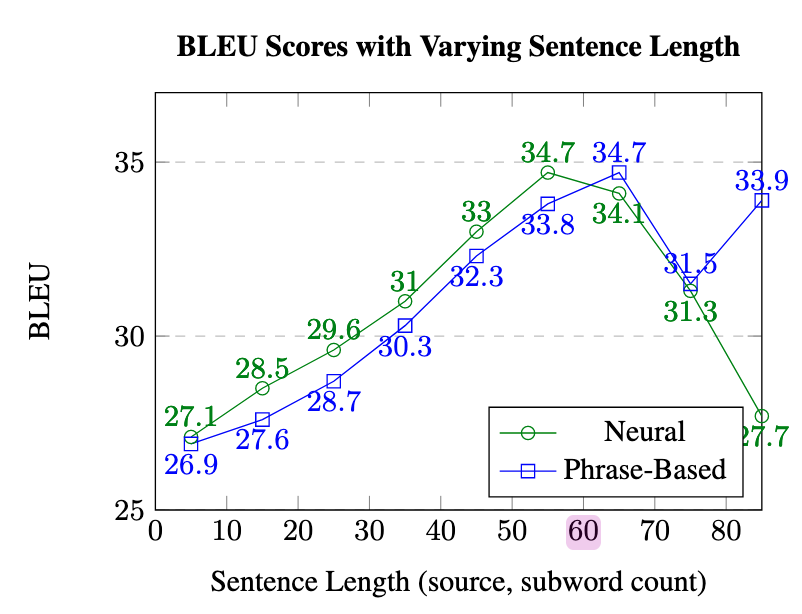
\includegraphics[width=0.95\textwidth]{img/bleusentencelength.png}}
    \centering
    \caption{Performance of SMT vs NMT on various sentence lengths from \normcite{koehn2017six}.}
    \label{img:bleusentlength}
\end{figure}


While NMT has been the primary technique used in various MT challenges, such as WMT, there are some advantages and disadvantages. According to \normcite{koehn2017six}, NMT suffers from the following phenomena:
\begin{itemize}
    \item In an out-of-domain scenario, NMT systems suffer more from quality loss than PBMT. The authors found that the model tends to sacrifice adequacy over fluency completely.

    \item NMT requires a large amount of data. It is problematic when low-resource languages are involved in the evaluation.

    \item NMT still shows weakness in the translation quality for low-frequency words despite its better performance. A similar problem also occurs in PBMT, where the model's performance suffers when low-frequency words occur in the sentence. The problem is especially apparent when the word is entirely unknown.

    \item Difficulties in translating long sentences. NMT can perform well in short sentences up to 60 words. However, longer sentences (80 and more tokens) show a lower quality of translation. \cref{img:bleusentlength} shows the performance of SMT and NMT on different sentence lengths.

    \item Model interpretability. As opposed to PBMT, it is not easy to interpret the behaviour of NMT due to the complexity of the model and its high number of parameters. Furthermore, the training of NMT is also non-deterministic due to random parameter initialization.
\end{itemize}

Despite its shortcomings, NMT is clearly and by far the current best approach. Among many other advantages, \normcite{machavcek2018enriching} mentioned that the difference is apparent in the output fluency. They mentioned that PBMT models suffer from double negation and translation in morphologically rich languages. These problems cause little to no problem at all in NMT models.

\section{Neural Machine Translation}
\label{sec:bm_nmt}
We define the translation problem used in this work as a mapping function $t$ from a given source language $S$ and target language $T$ from parallel corpus, that is $t : S \rightarrow T$. A parallel corpus is a set of sentence pairs in two different languages where one sentence in $T$ corresponds to its equivalent in language $S$. The goal of function $t$ is to find the highest probability of sentence $y \in T$ from $x \in S$, where $t(x) = argmax_y(p(y|x))$. The probability $p(y|x)$ is the probability estimation given by the NMT model.

The following sections show a quick overview of recent NMT models. They include architecture, advantages, and drawbacks.

\subsection{RNN Seq2Seq}
\normcite{sutskever2014sequence} proposes a sequence-to-sequence (seq2seq) model that employs Recurrent Neural Network (RNN) as the fundamental architecture. The architecture is a straightforward extension of the language model problem. Essentially, the model sequentially predicts the next word given all previous words while incorporating features obtained from the source language.

In MT, the approach is modified by using two similar model architectures for language $S$ and $T$. For language $S$ we call this component \texttt{encoder} and for $T$ we call it \texttt{decoder}.
The task of the \texttt{encoder} is to produce a vector representation of the input sentence from the source language $x \in S$. We define the input sentence as a sequence of tokens from a fixed vocabulary, i.e. the set of tokens permitted in the source language $\{x_1, x_2, ..., x_n\} \in x$. The tokens are then transformed into a vector representation by an embedding matrix. These representations consumed by an RNN result in a new representation that combines features from the embedding and its context. The \texttt{decoder} has a similar functionality as the \texttt{encoder} where it uses a sequence of tokens from $y \in T$ as its inputs. The \texttt{decoder} incorporates additional features from the last vector of the \texttt{encoder} and uses it throughout the entire sequence in the target language. For further illustration, we refer to \cref{img:rnnseq2seq}.

\begin{figure}[h]
    {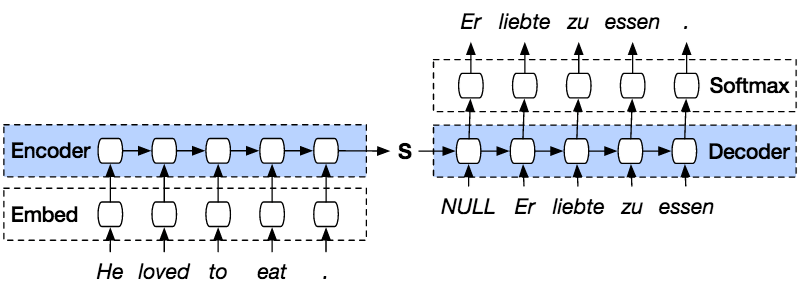
\includegraphics[width=0.95\textwidth]{img/rnnseq2seq.png}}
    \centering
    \caption{Illustration of seq2seq architecture from \normcite{johnson_2022}}
    \label{img:rnnseq2seq}
\end{figure}

\normcite{cho2014properties} found several disadvantages of using this variant of the seq2seq framework. The models' performance decreased when the length of the source sentence increased. From the previous paragraph, we recall that the \texttt{decoder} only uses the last vector of \texttt{encoder} as the additional feature.
The vector is a fixed-size vector whose size is defined prior to the training. Hence, the vector could be less informative when the source sentence grows due to the missing information that it has to sacrifice during the encoding. In essence, this framework forces the \texttt{encoder} to create a good representation by combining the features from all the words in the source sentence within a single vector with a limited size.

% \footnotetext[1]{Figure reprinted from \protect\url{https://www.guru99.com/seq2seq-model.html}.}

Furthermore, RNNs also suffer from another problem where the gradient can be extremely small or large. These problems are often mentioned as vanishing and exploding gradient problems. When the model's gradient is extremely small, RNNs can not learn from the data effectively and struggle, especially with long-range dependencies. On the other hand, when the gradient is extremely large, it can affect the weight parameters by moving them far away from the optimal space. This would disrupt the learning process and cause the model to fail to learn. This problem can happen in seq2seq architecture as we backpropagate the gradients from the last output of the \texttt{decoder} to the first input of the \texttt{encoder}.

\subsection{Seq2Seq with Attention}
The encoder-decoder model can be extended by jointly learning to translate and align words in the source language to the target language \citewithpar{bahdanau2015nmt}. This method learns to identify the most relevant sources of information in a source sentence and uses the encoder state vectors associated with the source positions to predict a target word.

\begin{figure}[h]
    {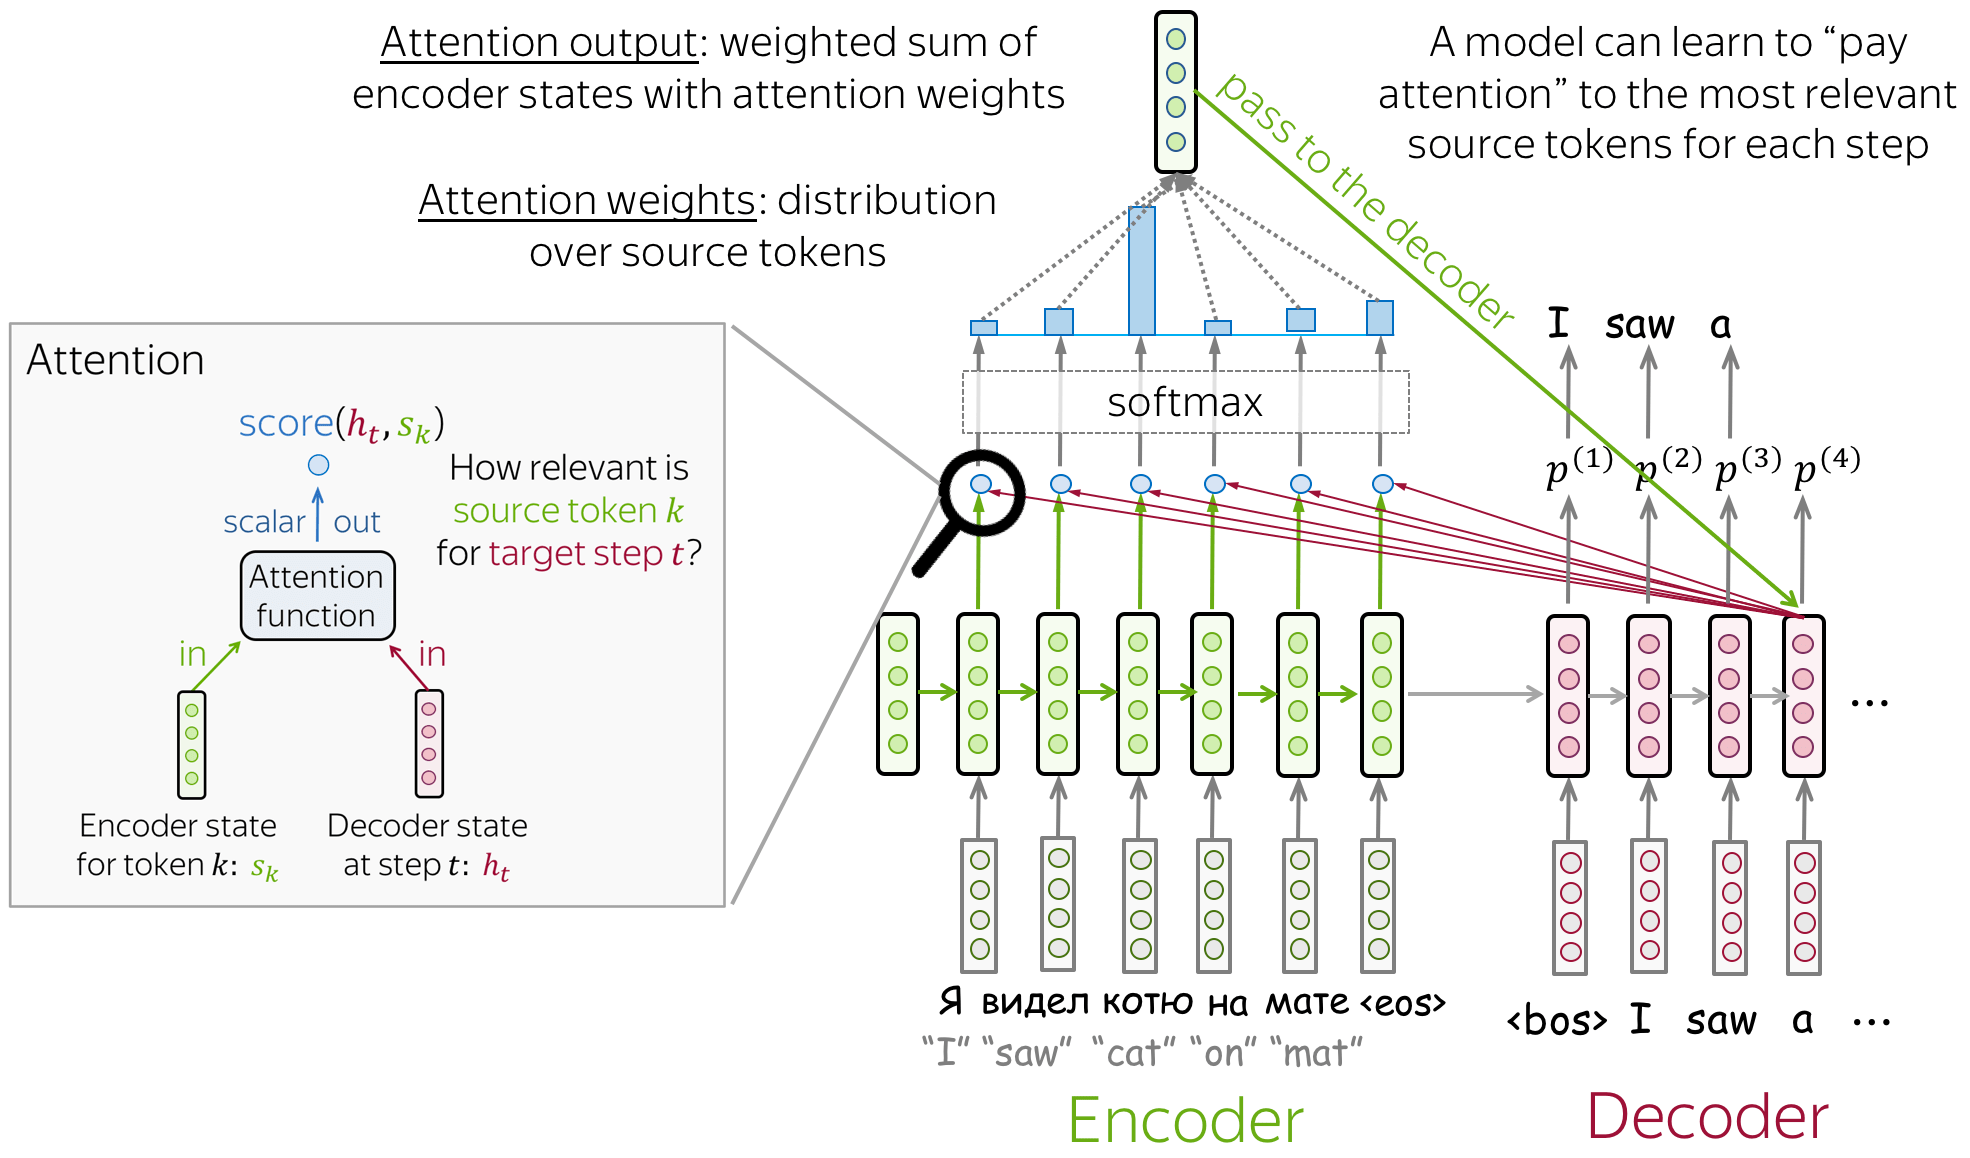
\includegraphics[width=0.95\textwidth]{img/attseq2seq.png}}
    \centering
    \caption{Illustration of seq2seq architecture with attention from \normcite{seq2seq_and_attention_2022}.}
    \label{img:attseq2seq}
\end{figure}

This method eliminates the need for a neural model to learn to squash the whole sentence into a fixed-length vector. Instead of encoding the whole sentence as proposed in the original method \citewithpar{sutskever2014sequence}, it is softly combining vectors from the source sentence that is deemed to contain the most relevant information to be used while decoding each word of the translated message. This allows the model to provide better predictions in long sentences. We can see the illustration of this architecture from \cref{img:attseq2seq}.

% \footnotetext[2]{Figure reprinted from \protect\url{https://lena-voita.github.io/nlp_course/seq2seq_and_attention.html}.}

The proposed approach achieves significantly better translation quality than the basic encoder-decoder model. The improvement is especially evident in longer sentences. The model shows comparable performance to or close to the phrase-based system in the En-Fr pair.

The motivation for this work is to identify the association between the decoder state and the input word. This attention method aims to measure the impact of word representation in the source sentence by looking at the strength of this association to produce the subsequent output word.

\subsection{Transformer}
Recurrent models such as RNN usually compute each token symbol of the input and produce output sequentially. During these sequential computations, they generate hidden states $h_t$ as a representation of the current position $t$. These hidden states take into consideration a combination of current input and the previous hidden state $h_{t-1}$. This behaviour implicitly forces the network to behave in a sequential manner and prevents parallelization within the training procedure. This parallelization becomes very important as the length of the input grows. Several works through factorization tricks \normcite{Kuchaiev2017FactorizationTF} and conditional computation \normcite{Shazeer2017OutrageouslyLN} have achieved notable improvements in reducing the computational time. However, it does not change the fact that the inherent sequential nature of the model remains.

To alleviate the sequential problem, \normcite{vaswani2017attention} proposed a new architecture called transformer. This new architecture avoids the recurrent nature of RNN entirely and only relies on the attention mechanism to provide dependencies between words in a sentence. It allows more parallelization and reduces significant training time to achieve a new state of the art in several tasks such as machine translation.

\begin{figure}[t]
    {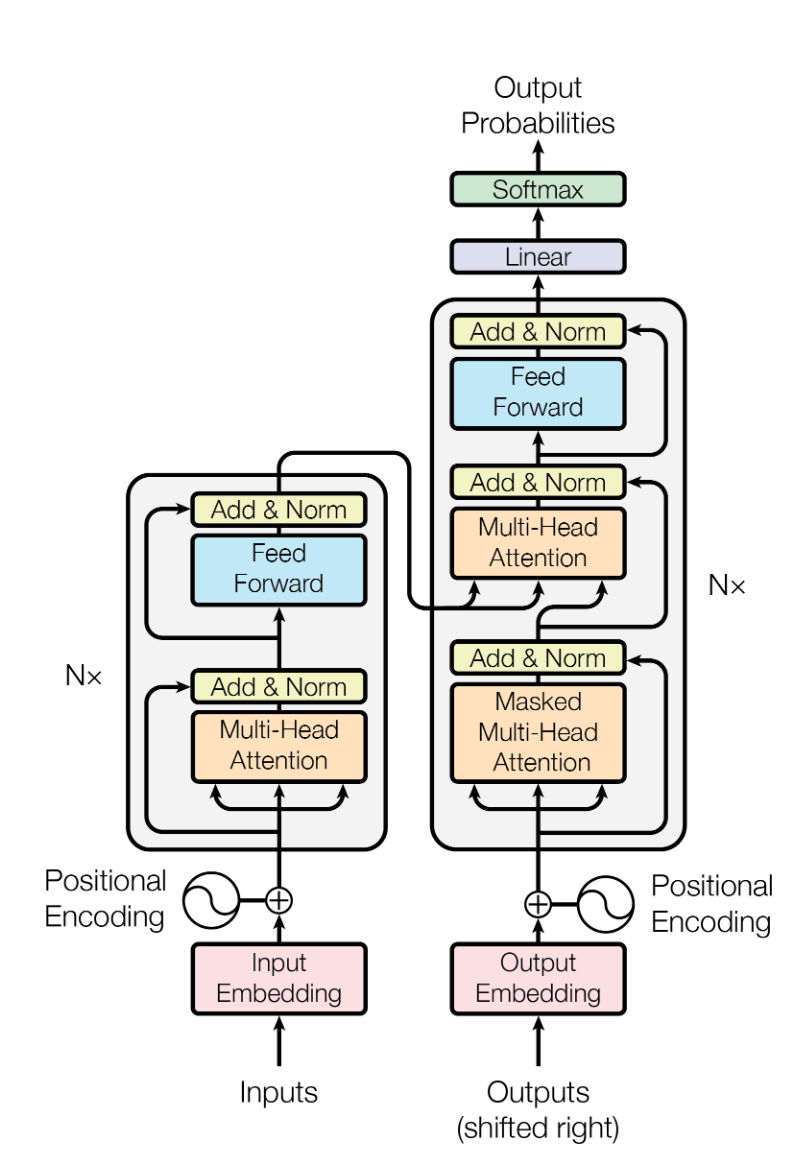
\includegraphics[width=0.55\textwidth]{img/transformer.png}}
    \centering
    \caption{Illustration of Transformer model. Figure reprinted from \normcite{vaswani2017attention}.}
    \label{img:transformer}
\end{figure}

We can refer to \cref{img:transformer} for illustration of the transformer architecture. The architecture again consists of two main components, an encoder and a decoder. The attention on the encoder side assigns an attention score to each word in the source sentence. The authors claim that compared to the sequential models, transformer is able to carry information between any pair of words in a single step and help the model reaches better quality while also improving the training speed. The authors further propose an additional attention layer on the decoder that refers to the representation in the encoder for a better context in a similar way as the attention in RNNs. This is helpful for tasks such as machine translation, where context from the source side is essential for the prediction.

Based on \normcite{liu2020understanding}, despite its contribution in leading many breakthroughs in NLP space, transformer requires non-trivial efforts in training the model. Contrary to the other neural layers such as recurrent neural network (RNN) and convolution neural network (CNN), optimization such as stochastic gradient descent (SGD) may converge to bad local optima if not tuned carefully. Furthermore, the warmup stage during training is crucial as it leads to severe consequences such as model divergence when it is omitted during training. We understand from this finding that training transformer and obtaining an optimal performance is not straightforward.

\section{Transfer Learning}
\label{sec:bm_tl}
Transfer learning (TL) focuses on transferring knowledge from one problem to a different but related problem. Transfer learning involves a source domain $D_S$ and a source task $T_S$, as well as a target domain $D_T$ and a target task $T_T$. We aim to learn and improve the target conditional distribution $P(Y_T|X_T)$ from $D_T$ by leveraging information from $D_S$ as well as $T_S$, where $D_S \neq D_T$, and/or $T_S \neq T_T$. We define $$Y_T$$ as the set of all target labels and $$X_T$$ as the document or sentence representations. For a better illustration on TL, we can refer to \cref{img:transfer_learning}.

\begin{figure}[h]
    {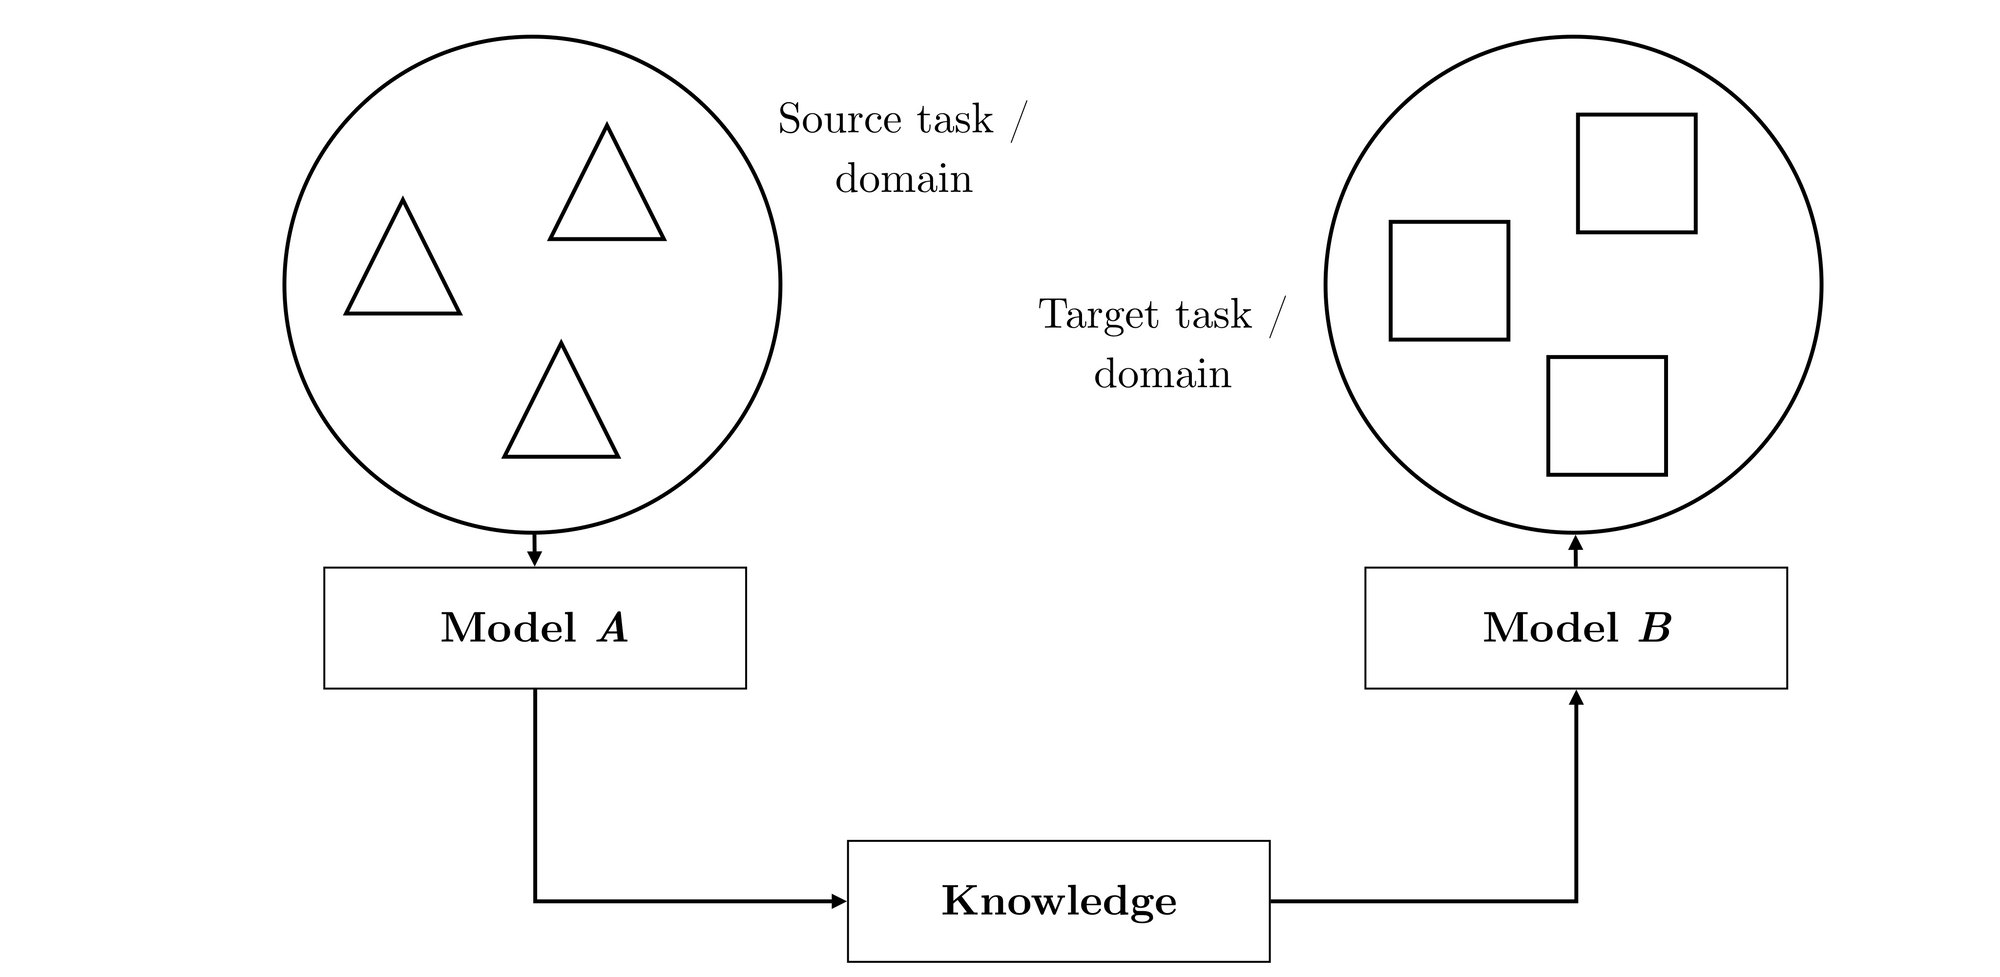
\includegraphics[width=0.95\textwidth]{img/transfer_learning_scenario.png}}
    \centering
    \caption{An illustration of transfer learning in different domain. Figure reprinted from \normcite{ruder2019transfer}.}
    \label{img:transfer_learning}
\end{figure}

\normcite{shavlik2010transfer} describe three ways of how transfer learning can
improve performance. Specifically:
\begin{itemize}
    \item Improving the initial performance at the beginning of training compared
          to a randomly initialized model when the tasks are similar;
    \item Shortening the time needed to reach the maximal performance;
    \item Improving the final performance level compared to training the model
          without the transfer
\end{itemize}

To some extent, we can see transfer learning as a way to initialize neural networks with more constraints than the usual definition of weights initialization. In weight initializations, we focus on initializing random weights for any neural network architecture. On the other hand, transfer learning is only applicable to a specific part of the neural network architecture within the same domain problem, i.e., we can only transfer weights from a network component to another network that uses the same component configuration, such as the number of neurons and layers. Domain problems can be defined as a category of problems such as computer vision, natural language processing, or speech recognition.
% As of this writing, we are not aware of any algorithm to perform transfer learning in different domain categories.

% For this work, we are specifically interested in two of the following categories of transfer learning: 1) Domain adaptation; 2) Sequential transfer learning. In the following sections, we will discuss the difference between these two categories.
For this work, we are specifically interested in conducting domain adaptation by learning the initial knowledge from a dataset with distribution $A$ and later using the knowledge as a new starting point for training in a different domain $B$. We achieve this by performing a sequential transfer learning technique, where we fine-tune the models that have already trained on distribution $A$ into distribution $B$. We will discuss the definition of domain adaptation and sequential transfer learning in the following sections to provide more details and examples of both techniques in MT.

\subsection{Domain Adaptation}
\label{sec:domain_adapt}
In the context of NMT, we can distinguish two categories of domain adaptation. The first category is domain adaptation in the linguistic sense, where we deal with the same language pairs but in different domains. For example, we pre-train a model in WMT data in German$\rightarrow$English pair and adapt IWSLT data within the same language. In the second category, we have multilingual adaptation, where we work with entirely different language pairs between the pre-training and the fine-tuning phase. For the scope of this thesis, we limit the problem to domain adaptation and only a single language. We choose not to perform further experiments on the multilingual adaptation as we want to isolate our study in understanding our proposed technique in one of the problems in transfer learning.

The goal of domain adaptation is to optimize a model that has been previously trained for a differrent domain. Models that are optimized on a specific genre (news, speech, medical, literature, and other) have higher accuracy than a system that is optimized for a more generic domain \citewithpar{gao2002improving,hildebrand2005adaptation}. This is due to the model's bias over the target domain. When the distribution of the training data is unbiased towards the test set in a particular target domain, we expect to reach a similar performance compared to the performance on a set held out from the training data. On the other hand, the performance will decline if the training data distribution is different.

In NMT, adaptation procedure involves training models over two different data distributions \citewithpar{luong2015stanford,Servan2016DomainSA,Chu2018ASO}. The models are first trained on an out-of-domain parallel corpus containing broad information. More in-domain training data is introduced to fine-tune the model when the first training has finished. We can see this as a form of transfer learning where the gained knowledge from the out-of-domain corpus is leveraged by the model while fine-tuning in the in-domain corpus.

There are two problems in domain adaptation found by \normcite{Freitag2016FastDA}:
\begin{itemize}
    \item The models are prone to over-fitting when the size of in-domain data is limited.
    \item The models suffer from catastrophic forgetting when they are fine-tuned. This means that the models' performance in the out-of-domain data will degrade while the performance on in-domain data may be improved.
\end{itemize}
A proposed solution from \normcite{Chu2017AnEC} addresses all these problems by mixed fine-tuning. Essentially, they combine the out-of-domain corpus and in-domain data when adapting the general model.

\subsection{Sequential Transfer Learning}
Based on \normcite{ruder2019transfer}, there are two existing strategies for applying pre-trained representations: feature-based and fine-tuning. The feature-based approach works by incorporating the representation as an additional feature to the models in the downstream tasks. The example of this approach can be found in ELMo \citewithpar{Peters2018DeepCW}. On the other hand, the fine-tuning approach employs the previously trained weights on the same model architecture in the downstream tasks. Several works such as BERT \citewithpar{devlin2018bert} and OpenAI GPT \citewithpar{Radford2018ImprovingLU} show fine-tuning provides a significant improvement compared to the feature-based approach. For that reason, we only consider the fine-tuning approach to train our model for this thesis.

Sequential transfer learning is a form of transfer learning that has led to the biggest improvements in NLP so far. In practice, we aim to perform pre-training to build decent vector representations from a large unlabelled text corpus and then adapt these representations to a target task with labelled data. For a better illustration, we refer to \cref{img:seq_tl}.

\begin{figure}[h]
    {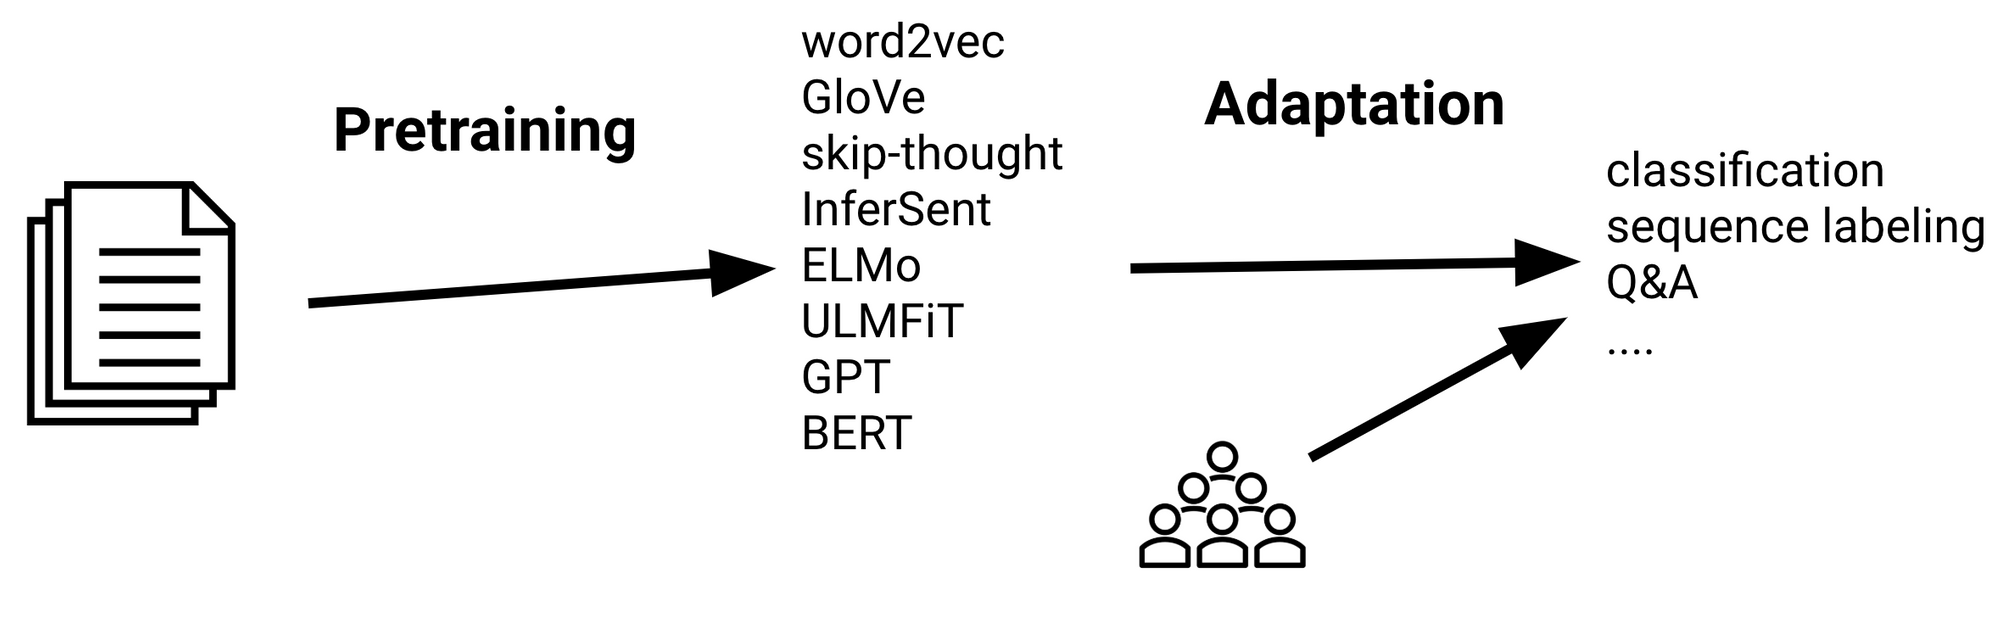
\includegraphics[width=0.95\textwidth]{img/sequential_tl.png}}
    \centering
    \caption{Illustration of sequential transfer learning. Figure reprinted from \normcite{ruder2019transfer}.}
    \label{img:seq_tl}
\end{figure}

In NLP, one of the most prominent examples of sequential transfer learning is pre-training with a language model objective. Language model pre-training has been shown as an effective objective in improving various NLP tasks \citewithpar{Dai2015SemisupervisedSL,Peters2018DeepCW,Radford2018ImprovingLU,Howard2018UniversalLM}. This includes sentence-level tasks in NLU such as natural language inference \citewithpar{Bowman2015ALA,Williams2018ABC} and sentence paraphrasing \normcite{Dolan2005AutomaticallyCA}. It also has been shown to improve performance in token-level tasks where models are expected to output another token, such as named entity recognition, question answering, and machine translation \citewithpar{Sang2003IntroductionTT,Rajpurkar2016SQuAD1Q}. In machine translation, the availability of high-quality parallel data can be a limitation to training good NMT models that can generate good output. Contextual knowledge such as the one from pre-trained models could be a good complement for NMT.

Although the language modelling task looks straightforward from a high-level overview, it is challenging for both machines and humans. For models to provide a solution, they must understand linguistic phenomena from both syntax and semantics as well as particular knowledge about the world. It has been shown that given enough data, enough computational power, and a large number of parameters, the model can provide a reasonable output \citewithpar{radford2018improving}. Several works have shown empirically that language modelling performs better than other pre-training tasks such as translation or autoencoding \citewithpar{Zhang2018LanguageMT,Wang2019CanYT}.

\subsubsection{BERT}
This section discusses BERT as one of the most prominent pre-trained models in NLP. It was proposed by \normcite{devlin2018bert} as they argue that the current language model objective restricts the power of the pre-trained representations, especially when applied for fine-tuning in the downstream tasks. There is a significant limitation from the conditional language models where it only performs unidirectional prediction. For example, we can not use RNN in left-to-right and right-to-left (bidirectional RNN) directions simultaneously, as each direction will provide answers for the other. This restriction can be harmful to sentence-level tasks. Especially in machine translation, it would be more beneficial to encode the sentence in both directions on the encoder part as we are only concerned with obtaining a good representation from the source sentence. Further illustration can be seen in \cref{img:bert}.

\begin{figure}[h]
    {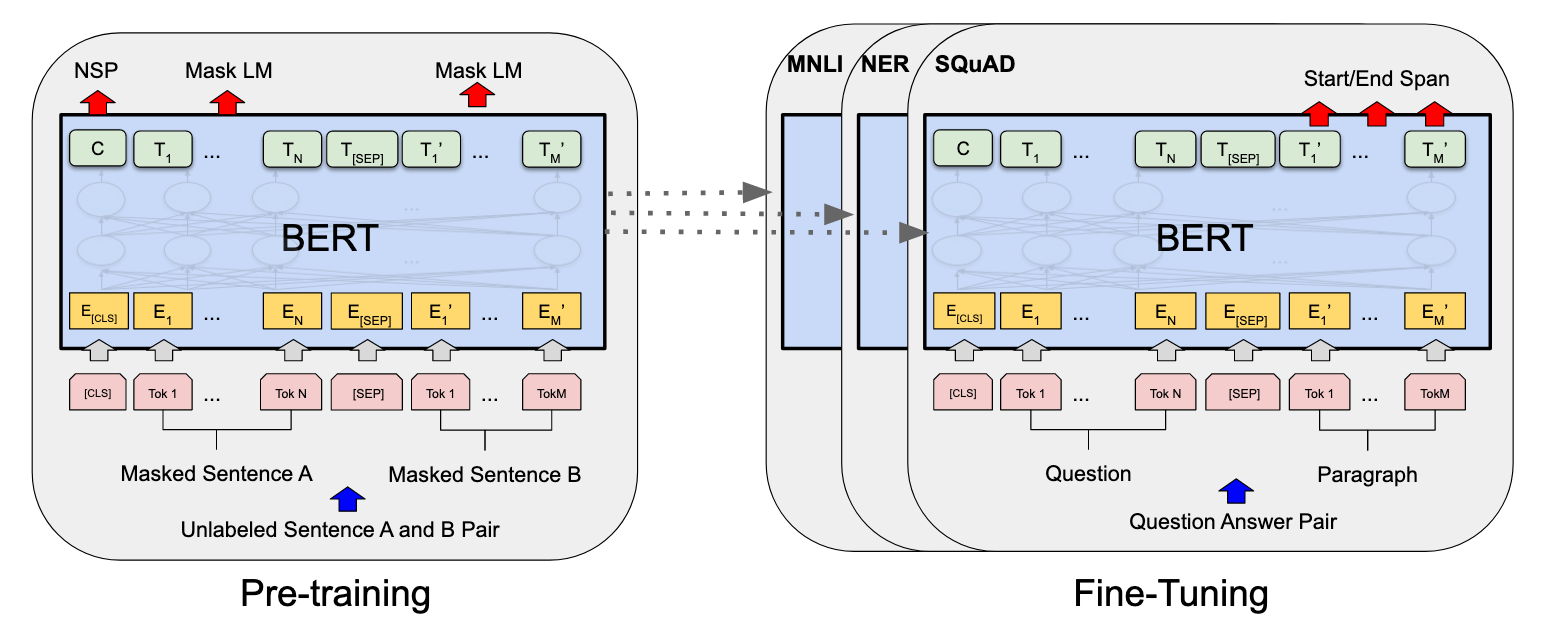
\includegraphics[width=0.95\textwidth]{img/bert.png}}
    \centering
    \caption{Illustration of BERT framework. Figure reprinted from \normcite{devlin2018bert}.}
    \label{img:bert}
\end{figure}

Despite its success in various NLU tasks, incorporating BERT in NLG remains challenging. \normcite{zhu2020incorporating} found that using pre-trained BERT as the initialization on the encoder side hurts the performance. An explanation for this is that fine-tuning BERT on a complex task requires extra care and may lead to the catastrophic forgetting problem \citewithpar{mccloskey1989catastrophic} of the pre-trained model. On the decoder side, there is a mismatch in initializing the component with BERT due to the conditional nature of the training objective. We understand that we can treat the objective of machine translation in the decoder as a conditional language model. This is different from BERT as it uses a bidirectional objective such as Masked Language Model (MLM). Furthermore, fine-tuning the full weights of the model is inefficient considering the enormous number of parameters in BERT. It is also tricky to fine-tune BERT with small datasets as the process can be unstable and fragile \citewithpar{Lee2020MixoutER}.

\section{Adapters}
\label{sec:bm_adapters}
An adapter is a lightweight layer inserted between the layers of a pre-trained transformer network, and it is fine-tuned on the adaptation corpus. The adapters were proposed by \normcite{houlsby2019parameter} as an alternative to fine-tuning. In this work, we follow the architecture similar to the work of \normcite{bapna2019simple} as it is simpler to implement and has been adopted in other works \citewithpar{pfeiffer2020madx,ruckle2020adapterdrop,pfeiffer2021adapterfusion}. Specifically, we follow the adapter implementation of \normcite{pfeiffer2020madx} because they have already performed an extensive hyperparameter search to find the best combination of the position and the number of adapters within a single layer, the position of residual connections, the bottleneck residual factors, as well as the non-linearity function within the bottleneck adapter layer within each transformer layer.

Following \normcite{pfeiffer2020madx}, adapter is defined with the following formulation

$$A_l(h_l, r_l) = U_l(ReLU(D_l(LA_l))) + r_l $$

$A_l$ is the adapter incorporated at layer $l$, $D_l$ is a down projection layer $D \in R^{h \times d}$ where $h$ is the dimension of the current layer and $d$ is the adapter dimension, $U_l$ is an up projection layer $U \in R^{d \times h}$, and $r_l$ is the residual connection from the previous layer, both $h$ and $l$ are larger than $d$. We can refer to \cref{img:adapters} for an illustration of the adapter bottleneck layer and how they are incorporated to the Transformer architecture.

\begin{figure}[h]
    {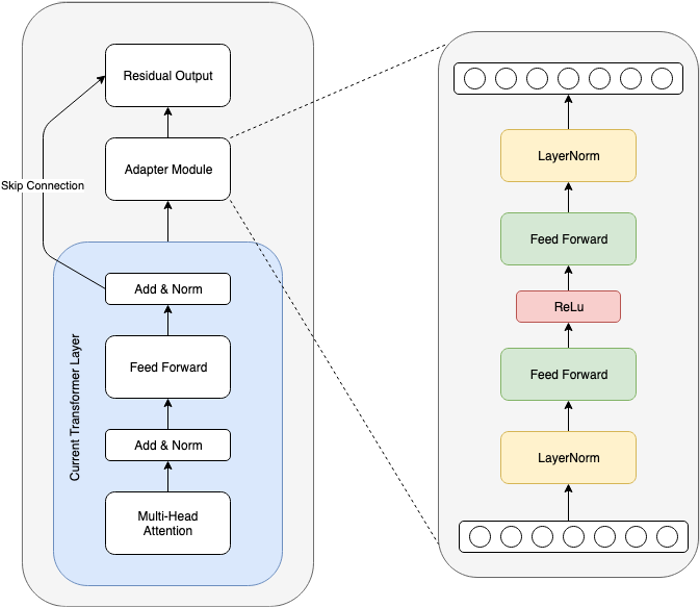
\includegraphics[width=0.75\textwidth]{img/adapter_module.png}}
    \centering
    \caption{Illustration of Adapters.}
    \label{img:adapters}
\end{figure}

There are several problems in fine-tuning that adapters are trying to solve:
\begin{itemize}
    \item The number of parameters in the state-of-the-art NMT has been increasing \citewithpar{Shazeer2018MeshTensorFlowDL,Bapna2018TrainingDN,Huang2019GPipeET}, and performing fine-tuning on all parameters is too costly.
    \item Fine-tuning the whole network weights demands meticulous hyper-parameter tuning during the adaptation process, and it is prone to over-fitting \citewithpar{Sennrich2016ImprovingNM,Barone2017RegularizationTF}.
    \item \normcite{Lee2020MixoutER} suggests that catastrophic forgetting leads to instability during fine-tuning.
    \item \normcite{Mosbach2021OnTS} suggests gradient vanishing also contributes in instability during fine-tuning.
    \item The high capacity model intensifies the sensitivity to both hyper-parameter and over-fitting.
\end{itemize}

\normcite{han2021robust} show that fixing the pre-trained layers and only fine-tuning adapter modules improves the model's stability on various random seeds, enhances adversarial robustness, and leads to a better final performance. We can see \cref{img:adapters_instability} for the difference between models that were trained with (cluster on the right) and without adapters (cluster on the left) on different pre-training and fine-tuning iterations. The fine-tuned models with adapters show more stability than the ones that were not using adapters. The pre-training models use the same architecture and network configurations during the training but use different iterations to stop the training.

\begin{figure}[h]
    {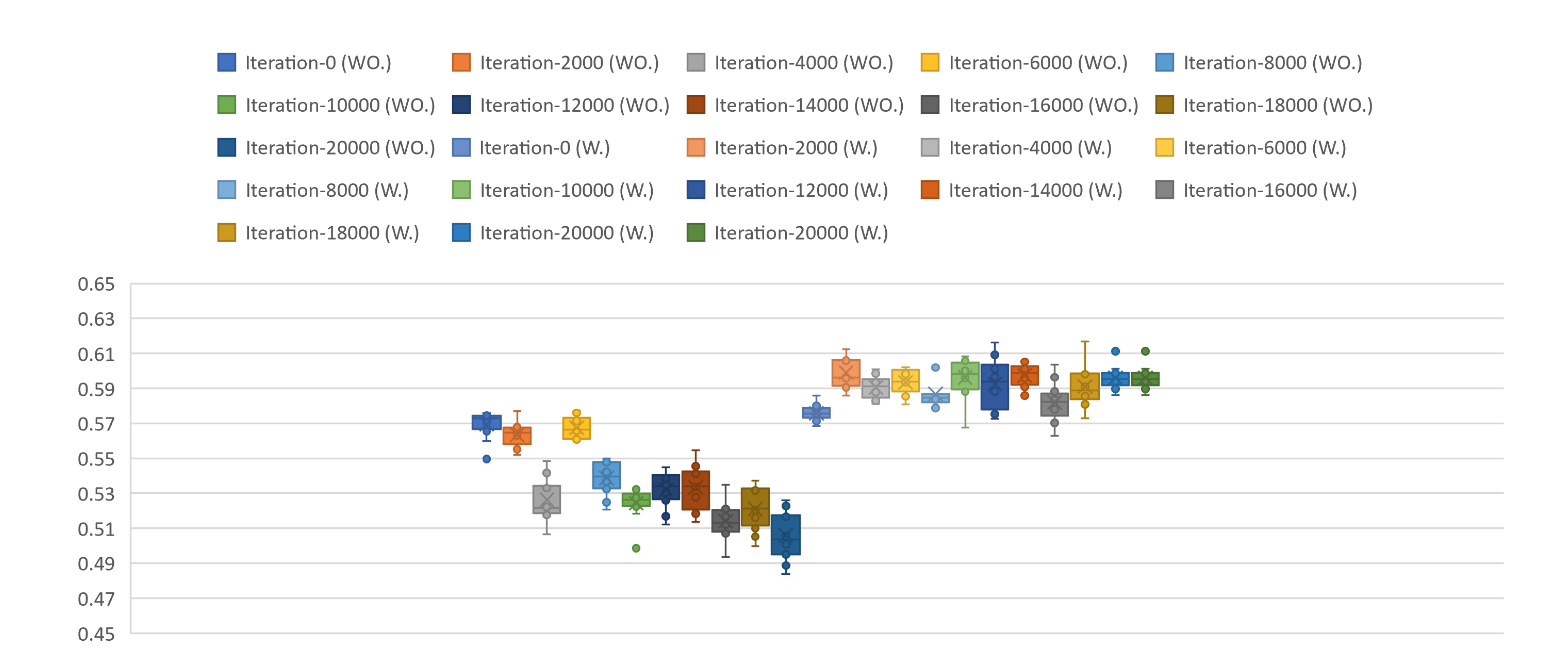
\includegraphics[width=0.95\textwidth]{img/adapters_instability.png}}
    \centering
    \caption{Illustration of adapters instability. ``W'' represents the models that use adapters and ``WO'' represents the models that do not use adapters. Figure reprinted from \cite{han2021robust}.}
    \label{img:adapters_instability}
\end{figure}